\documentclass[a4paper,12pt]{article}

% Paquetes básicos
\usepackage[utf8]{inputenc}
\usepackage[T1]{fontenc}
\usepackage[spanish]{babel}
\usepackage{graphicx}
\usepackage{xcolor}
\usepackage{lipsum}
\usepackage{geometry}
\geometry{top=3cm, bottom=3cm, left=2.5cm, right=2.5cm}

% Paquetes para diseño
\usepackage{titlesec}
\usepackage{fancyhdr}
\usepackage{amsmath}
\usepackage{amssymb}
\usepackage{hyperref}

% Paquetes para el entorno lstlisting
\usepackage{listings}
\usepackage{inconsolata}

%encabezado y pie de página nivel profesional
\usepackage{fancyhdr}
\pagestyle{fancy}
\fancyhf{}
\fancyhead[L]{\leftmark}
\fancyhead[R]{\rightmark}
\fancyfoot[C]{\thepage}
\fancyfoot[R]{\textbf{(UGR)} \today}
\renewcommand{\headrulewidth}{0.4pt}
\renewcommand{\footrulewidth}{0.4pt}
\setlength{\headheight}{15pt}
\setlength{\headsep}{10pt}
\setlength{\footskip}{20pt}
\usepackage{truncate}
\fancyhead[L]{\truncate{0.5\headwidth}{\leftmark}}
\fancyhead[R]{\truncate{0.5\headwidth}{\rightmark}}
\usepackage{mathpazo}
\usepackage{tcolorbox}


% Paquete para fondo
\usepackage{background}
\usepackage{float}

% Configuración de lstlisting
\lstset{
    inputencoding=utf8,          % Permite UTF-8
    extendedchars=true,          % Reconoce caracteres extendidos
    literate=                    % Configuración manual para tildes y símbolos
        {á}{{\'a}}1
        {é}{{\'e}}1
        {í}{{\'i}}1
        {ó}{{\'o}}1
        {ú}{{\'u}}1
        {ñ}{{\~n}}1
        {Á}{{\'A}}1
        {É}{{\'E}}1
        {Í}{{\'I}}1
        {Ó}{{\'O}}1
        {Ú}{{\'U}}1
        {Ñ}{{\~N}}1
        {¿}{{\textquestiondown}}1
        {¡}{{\textexclamdown}}1,
    basicstyle=\ttfamily,        % Fuente monoespaciada
    breaklines=true,             % Habilita salto de línea automático
    frame=single,                % Marco alrededor del código
    backgroundcolor=\color{gray!10}, % Fondo gris claro
    keywordstyle=\color{blue},   % Color para palabras clave
    commentstyle=\color{green},  % Color para comentarios
    stringstyle=\color{red}      % Color para strings
}
\lstdefinestyle{customcpp}{
    language=C++,                % Lenguaje de programación
    showspaces=false,            % No mostrar espacios
    showtabs=false,              % No mostrar tabulaciones
    tabsize=4,                   % Tamaño de tabulación
    showstringspaces=false,      % No mostrar espacios en strings
    numbers=left,                % Números de línea a la izquierda
    numberstyle=\tiny\color{gray}, % Estilo de los números de línea
    numbersep=5pt,               % Separación de los números de línea
    stepnumber=1,                % Mostrar número en cada línea
    basicstyle=\ttfamily\footnotesize, % Estilo básico del código
    keywordstyle=\bfseries\color{blue}, % Estilo de las palabras clave
    commentstyle=\itshape\color{green!50!black}, % Estilo de los comentarios
    stringstyle=\color{red},     % Estilo de los strings
    identifierstyle=\color{black}, % Estilo de los identificadores
    % procnamekeys={def,class},    % Palabras clave para nombres de funciones
    morekeywords={constexpr,nullptr,size_t}, % Más palabras clave
    emph={int,char,double,float,unsigned}, % Palabras a enfatizar
    emphstyle=\color{magenta},   % Estilo de las palabras enfatizadas
    backgroundcolor=\color{gray!10}, % Color de fondo
    frame=shadowbox,             % Marco con sombra
    rulesepcolor=\color{gray},   % Color de la línea de separación
    breakatwhitespace=false,     % No cortar en espacios en blanco
    breaklines=true,             % Cortar líneas largas
    captionpos=b,                % Posición del título (abajo)
    escapeinside={(*@}{@*)},     % Delimitadores para escapar a LaTeX
    morecomment=[l][\color{magenta}]{\#}, % Comentarios de una línea
    morecomment=[s][\color{orange}]{/*}{*/}, % Comentarios multilínea
    morestring=[b]",             % Strings entre comillas dobles
    morestring=[b]'              % Strings entre comillas simples
}

% Configuración de título
\titleformat{\section}{\normalfont\Large\bfseries}{\thesection}{1em}{}

% Información del documento
\title{
    \vspace{-2cm}
    
\includegraphics[width=0.3\textwidth]{images/etsiit.png} \\ % Cambia el logo si es necesario
    \LARGE Ingeniería Informática + ADE\\
    \large Universidad de Granada (UGR)\\[1cm]
}
\author{\textbf{Autor:} Ismael Sallami Moreno}
\date{\textbf{Asignatura:} Apuntes Fundamentos de redes (FR)\\[1cm]}

% Configuración del fondo
\backgroundsetup{
    scale=1,
    color=black,
    opacity=0.2,
    angle=0,
    position=current page.south,
    vshift=0pt,
    hshift=0pt,
    contents={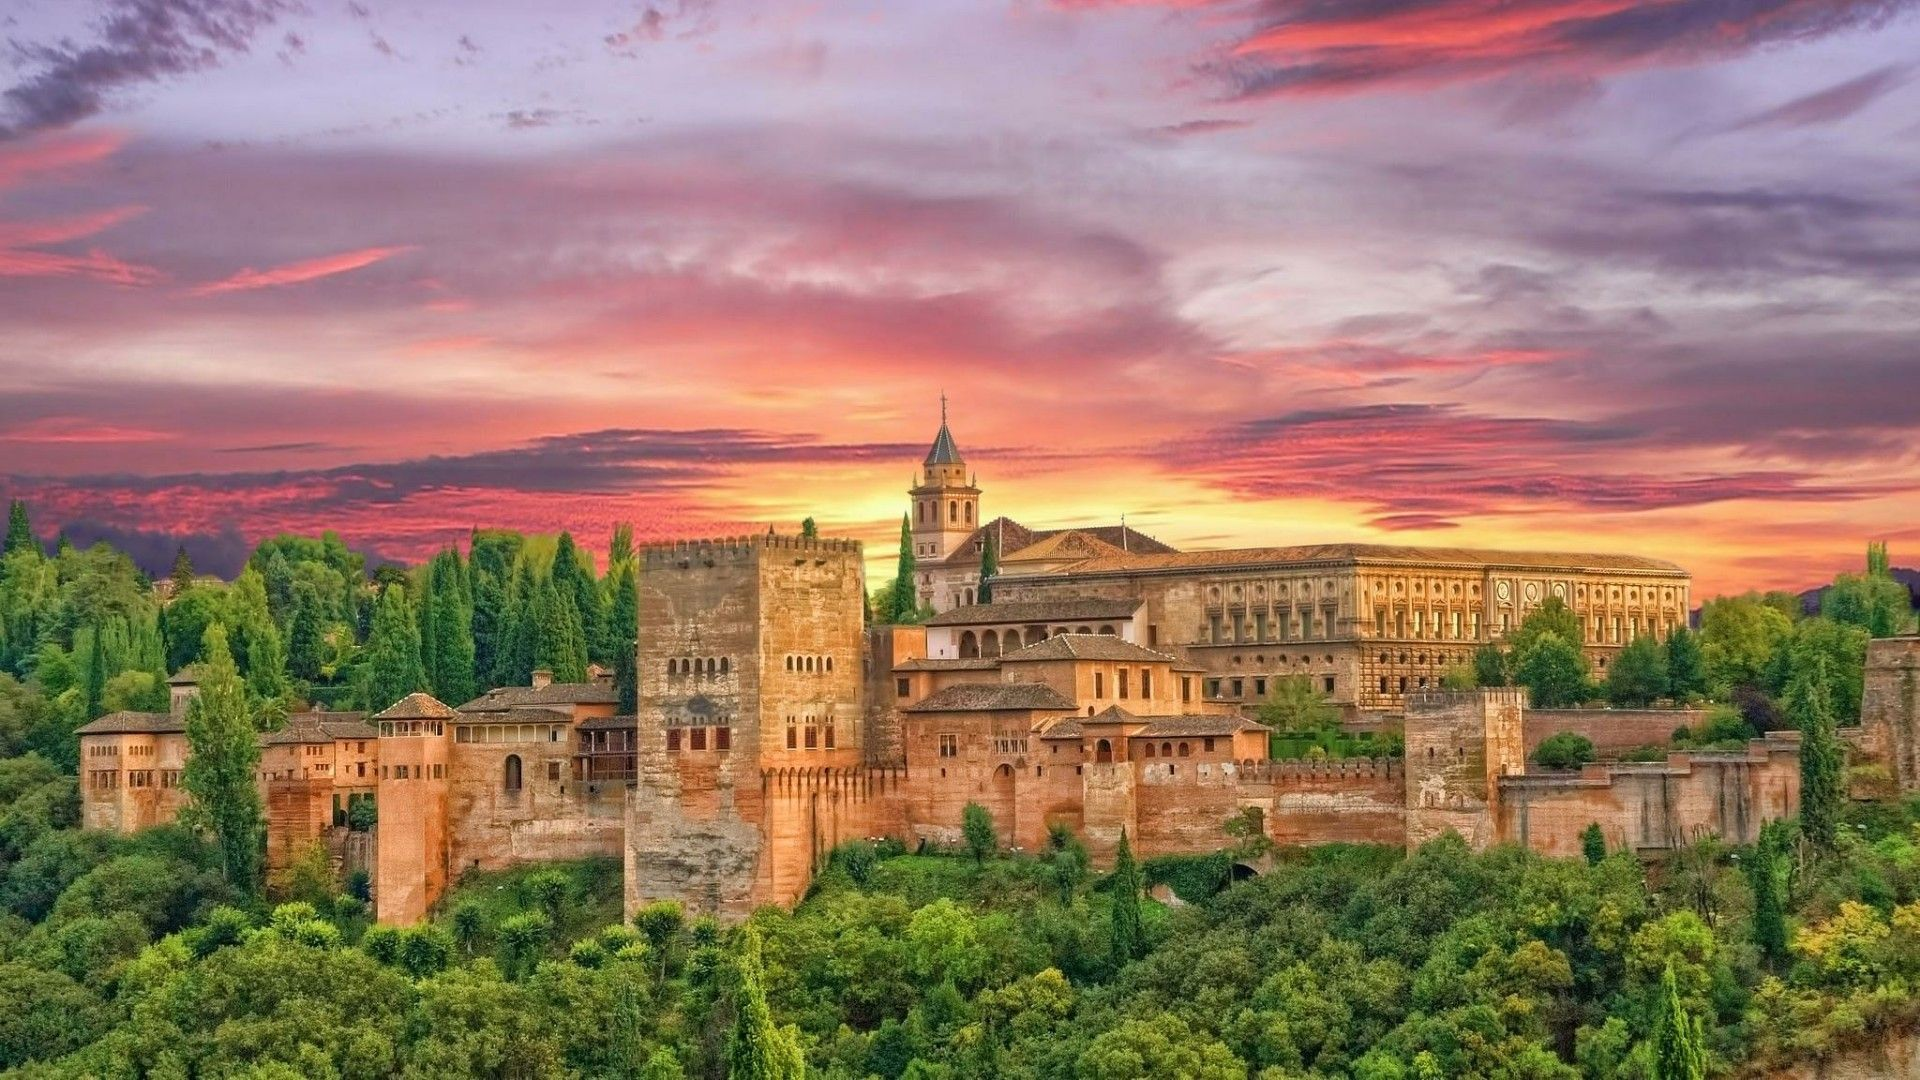
\includegraphics[width=\paperwidth,height=\paperheight,keepaspectratio]{images/granada.jpg}}
}

% Inicio del documento
\begin{document}

% Portada
\maketitle
\thispagestyle{empty}

\begin{center}
    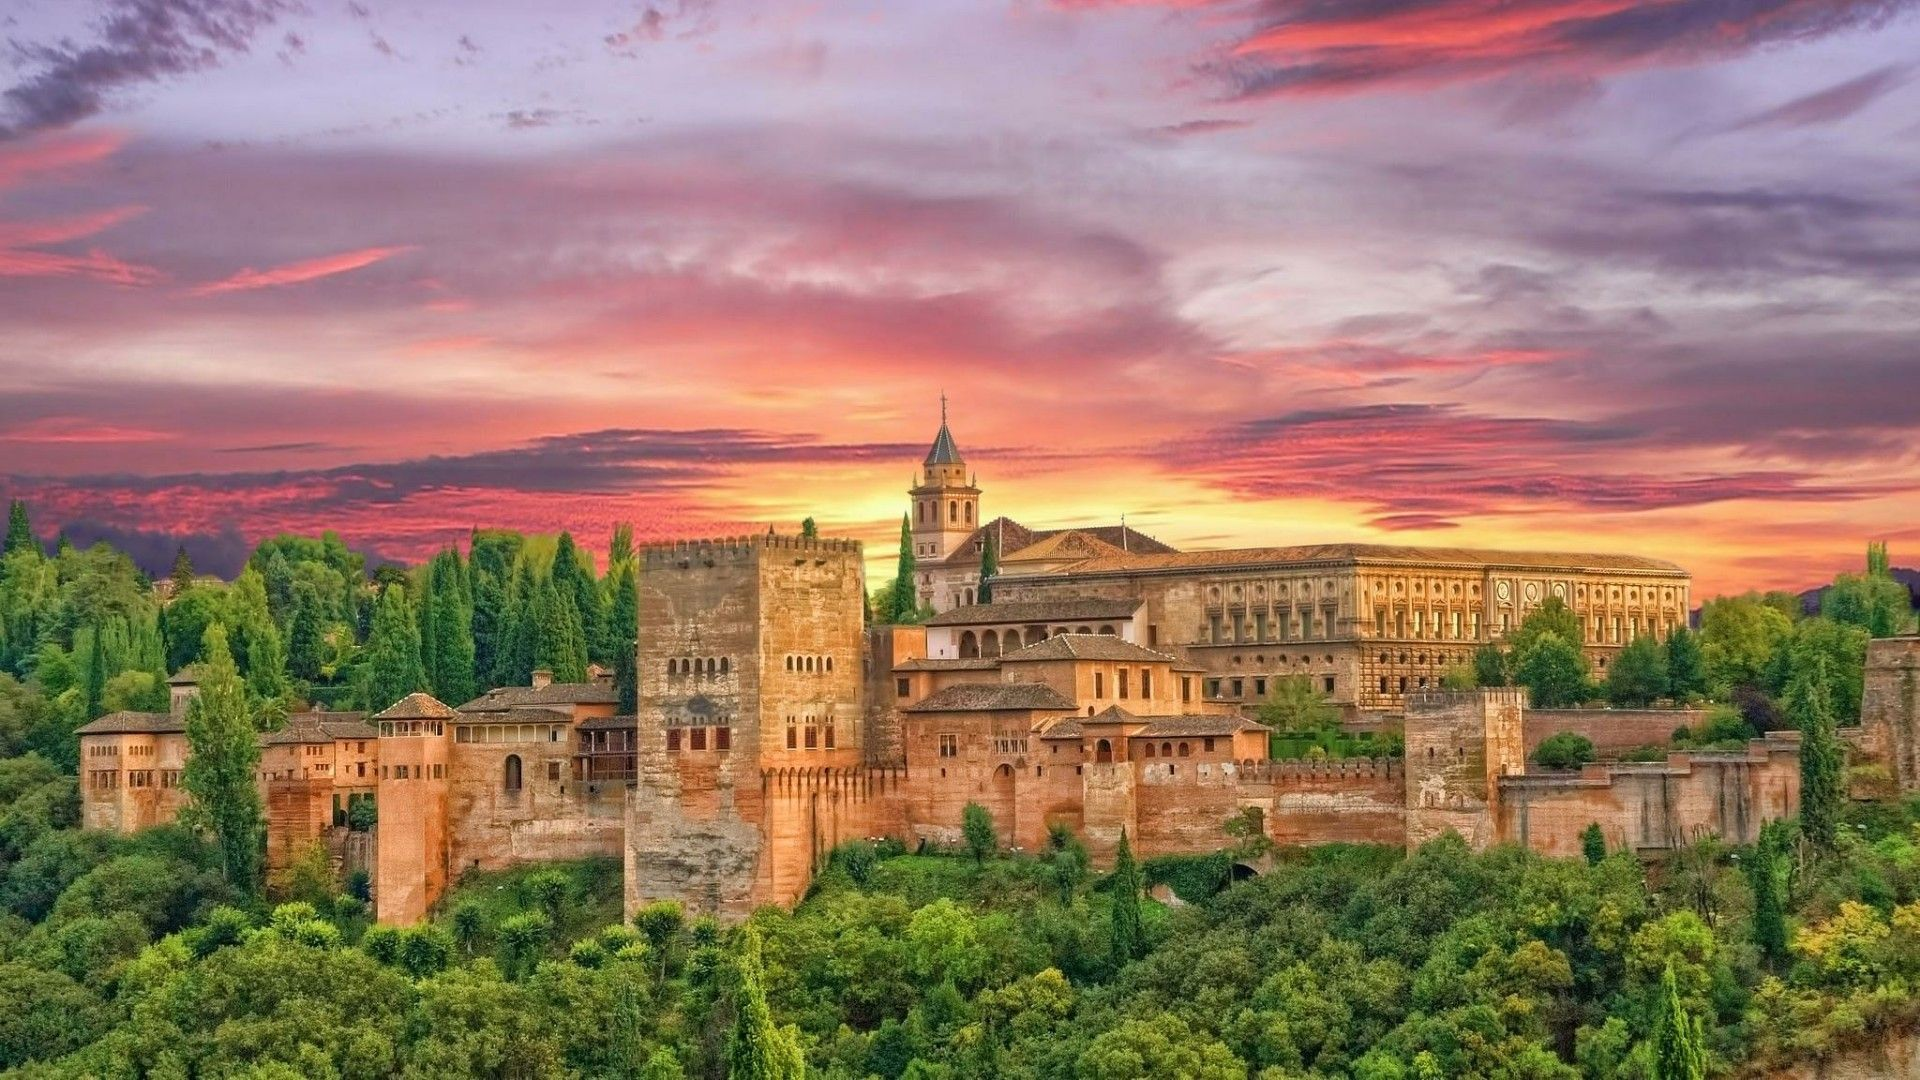
\includegraphics[width=\textwidth,height=0.4\textheight,keepaspectratio]{images/granada.jpg} \\ % Añade tu imagen de fondo
    \vfill
\end{center}

\newpage

% Índice (opcional)
\tableofcontents
\newpage

\section{Tema 1: Introducción a los fundamentos de las redes}

\subsection{Sistemas de comunicación y redes}

Se define por un sistema de comunicación  a la infraestructura (hard y soft) que permite el intercambio de la información. La información es el conjuntos de datos que tienen un significado. Y por red entendemos al sistema de comunicación con sistemas finales y autónomos, que tiene capacidad de procesar la información. facilitando el intercambio efizar y transparente de información.\\

La motivación para usar redes es la posibilidad de compartir recursos, la escalabilidad, fiabilidad, robustez, duplicidad y el ahorro de costes.\\

Características de una red, ya sea de computadores, de móviles, etc es la autonomía, la interconexión y el intercambio de información de manera eficaz y transparente.\\

Los elementos de una red son:
\begin{itemize}
    \item Hosts: sistemas finales, es decir, las termiles. Además son autónomos.
    \item Subred: es una infraestructura para el transporte de información. Esta consta de líneas de transmisión y nodos de elementos de comunicación, como pueden ser routers, switches, etc.
\end{itemize}

Ejemplos de medios de transmisión:
\begin{itemize}
    \item Cable coaxial
    \item Cable por trenzado: UTP, STP, FTP
    \item Fibra óptica
\end{itemize}

\subsubsection*{Topologías de redes: patrón de interconexión entre sus nodos}

\begin{itemize}
    \item Física vs lógica
    \item Tipos:
    \begin{itemize}
        \item En bus 
        \item En anillo
        \item En estrella
        \item En malla
        \item En árbol
        \item En híbrida
    \end{itemize}
\end{itemize}

\subsection{Clasificación de las redes}

\begin{itemize}
    \item Según su tamaño: PAN (personal), LAN(local), MAN(matropolitano), WAN:
    \begin{itemize}
        \item PAN (Personal Area Network): Es una red utilizada para la comunicación entre dispositivos de una persona, típicamente en un rango de unos pocos metros. Ejemplos incluyen la conexión entre un teléfono móvil y un auricular Bluetooth.
        \item LAN (Local Area Network): Es una red que cubre un área geográfica pequeña, como una casa, oficina o edificio. Permite la interconexión de dispositivos como computadoras, impresoras y otros equipos dentro de un área limitada.
        \item MAN (Metropolitan Area Network): Es una red que abarca una ciudad o una gran área metropolitana. Se utiliza para conectar varias LANs dentro de una ciudad, proporcionando alta velocidad y conectividad eficiente.
        \item WAN (Wide Area Network): Es una red que cubre un área geográfica extensa, como un país o incluso continentes. Las WANs permiten la comunicación y el intercambio de datos entre dispositivos ubicados en diferentes lugares geográficos. Internet es el ejemplo más conocido de una WAN.
    \end{itemize}
    \item Según la tecnologia de transmisión:
    \begin{itemize}
        \item Difusión: En este tipo de red, un solo nodo transmite datos a todos los demás nodos en la red. Un ejemplo común es la red de televisión por aire.
        \item Punto a punto: En este tipo de red, los datos se transmiten directamente entre dos nodos específicos. Un ejemplo común es una conexión telefónica.
    \end{itemize}
    \item Según el tipo de transferencia entre datos:
    \begin{itemize}
        \item \textbf{Simplex}: Es un modo de comunicación unidireccional, donde la información solo puede ser enviada en una dirección. Un ejemplo común es la transmisión de televisión.
        \item \textbf{Half-duplex}: Es un modo de comunicación bidireccional, pero no simultánea. Esto significa que la información puede ser enviada en ambas direcciones, pero no al mismo tiempo. Un ejemplo es un walkie-talkie.
        \item \textbf{Full-duplex}: Es un modo de comunicación bidireccional y simultánea. Esto significa que la información puede ser enviada y recibida al mismo tiempo. Un ejemplo es una llamada telefónica.
    \end{itemize}
\end{itemize}

\subsubsection{Nomenclatura típica en figuras}
    \begin{figure}[H]
        \centering
        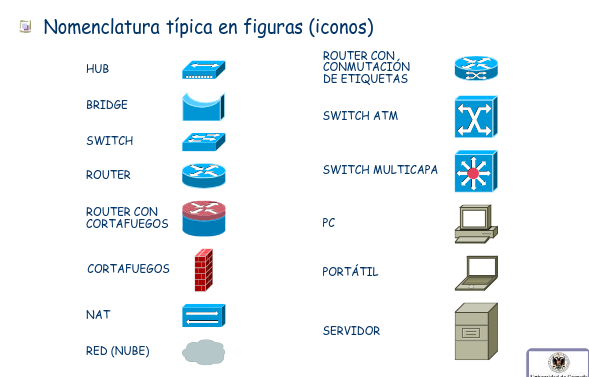
\includegraphics[width=0.8\textwidth]{images/nomenclatura.png}
    \end{figure}

\begin{itemize}
    \item \textbf{HUB}: Dispositivo que conecta múltiples computadoras en una red local. Reenvía los datos recibidos a todos los dispositivos conectados.
    \item \textbf{ROUTER}: Encargado de dirigir paquetes de datos entre diferentes redes. Se utiliza para conectar redes locales a Internet o a otras redes.
    \item \textbf{SWITCH}: Dispositivo que conecta múltiples dispositivos en una red local, pero a diferencia de un HUB, envía los datos solo al dispositivo destinatario, mejorando la eficiencia.
    \item \textbf{BRIDGE}: Permite conectar dos redes locales separadas y filtrar el tráfico entre ellas en función de la dirección MAC.
    \item \textbf{SWITCH ATM}: Diseñado para redes que usan la tecnología de Modo de Transferencia Asíncrona (ATM), que transporta datos en celdas de longitud fija.
    \item \textbf{SWITCH MULTICAPA}: Similar a un switch, pero con la capacidad de operar en varias capas del modelo OSI, como la capa de red (3) y la capa de enlace (2).
    \item \textbf{ROUTER CON CORTAFUEGOS}: Combina las funciones de un router y un cortafuegos para proporcionar seguridad y dirigir tráfico en redes.
    \item \textbf{RED (NUBE)}: Representación abstracta de una red o conjunto de redes, que típicamente se utiliza para denotar servicios en la nube o conexiones externas.
    \item \textbf{NAT (Network Address Translation)}: Tecnología que permite que varios dispositivos compartan una única dirección IP pública mediante la traducción de direcciones.
    \item \textbf{PC}: Computadora personal que actúa como un host en una red.
    \item \textbf{SERVIDOR}: Computadora diseñada para proveer servicios a otros dispositivos en la red, como archivos, aplicaciones o datos.
    \item \textbf{PORTÁTIL}: Computadora portátil que también puede funcionar como host en una red.
    \item \textbf{CORTAFUEGOS}: Dispositivo o software diseñado para proteger redes bloqueando o permitiendo el tráfico en función de reglas predefinidas.
    \item \textbf{ROUTER CON CONMUTACIÓN DE ETIQUETAS}: Router que utiliza conmutación basada en etiquetas, como MPLS (Multiprotocol Label Switching), para optimizar el enrutamiento.
\end{itemize}

Los que debemos de saber dibujar son: \textbf{HUB, SWITCH, ROUTER.}

\subsubsection{Estructura y Elementos de una Red según Kurose y Ross}

La estructura y los elementos de una red están compuestos por diversos componentes que trabajan juntos para permitir la comunicación eficiente entre sistemas finales. Según Kurose y Ross, estos son los elementos principales:

\begin{itemize}
    \item \textbf{Hosts (Sistemas finales)}: 
    Dispositivos autónomos que actúan como origen o destino de la comunicación en una red. Los hosts pueden ser computadoras, servidores, dispositivos móviles o cualquier terminal que procese información.

    \item \textbf{Subred}: 
    La infraestructura que permite el transporte de información entre los sistemas finales. Dentro de una subred, encontramos dos elementos clave:
    \begin{itemize}
        \item \textbf{Líneas de transmisión}: Canales físicos o lógicos que transportan los datos entre los nodos de la red. Estos pueden ser cables de par trenzado, fibra óptica, enlaces inalámbricos, entre otros.
        \item \textbf{Nodos o elementos de conmutación}: Dispositivos intermedios como \textit{routers} o \textit{switches}, que se encargan de redirigir y gestionar el tráfico de datos dentro de la subred.
    \end{itemize}
\end{itemize}

Estos elementos se combinan para formar una red que facilita la interconexión y el intercambio de información de manera eficiente y transparente.

\subsection{Diseño y estandarización de redes}

Debemos de mencionar el \textit{Modelo de referencia} que engloba la defición de capas y de las funcionalidades. Para el diseño se deben de seguir ciertos apéndices:
\begin{itemize}
    \item Funcionalidades que son distintas deben de estar en capas distintas.
    \item Minimizar el flujo de información entre capas.
\end{itemize}

\subsubsection{Modelos OSI, TCP/IP y el concepto de RFC}

\subsubsection*{Modelos OSI y TCP/IP}

\begin{itemize}
    \item \textbf{OSI (Open Systems Interconnection)}: 
    Este modelo, desarrollado por la \textit{International Organization for Standardization (ISO)}, divide las comunicaciones de red en siete capas funcionales. Estas capas, que van desde la física hasta la aplicación, proporcionan un marco conceptual para la interoperabilidad entre sistemas.

    \item \textbf{TCP/IP (Transmission Control Protocol/Internet Protocol)}: 
    Es el modelo práctico utilizado para las comunicaciones en Internet, desarrollado por el \textit{Internet Engineering Task Force (IETF)}. Se compone de cuatro capas que se alinean funcionalmente con el modelo OSI.
\end{itemize}

\begin{figure}[H]
    \centering
    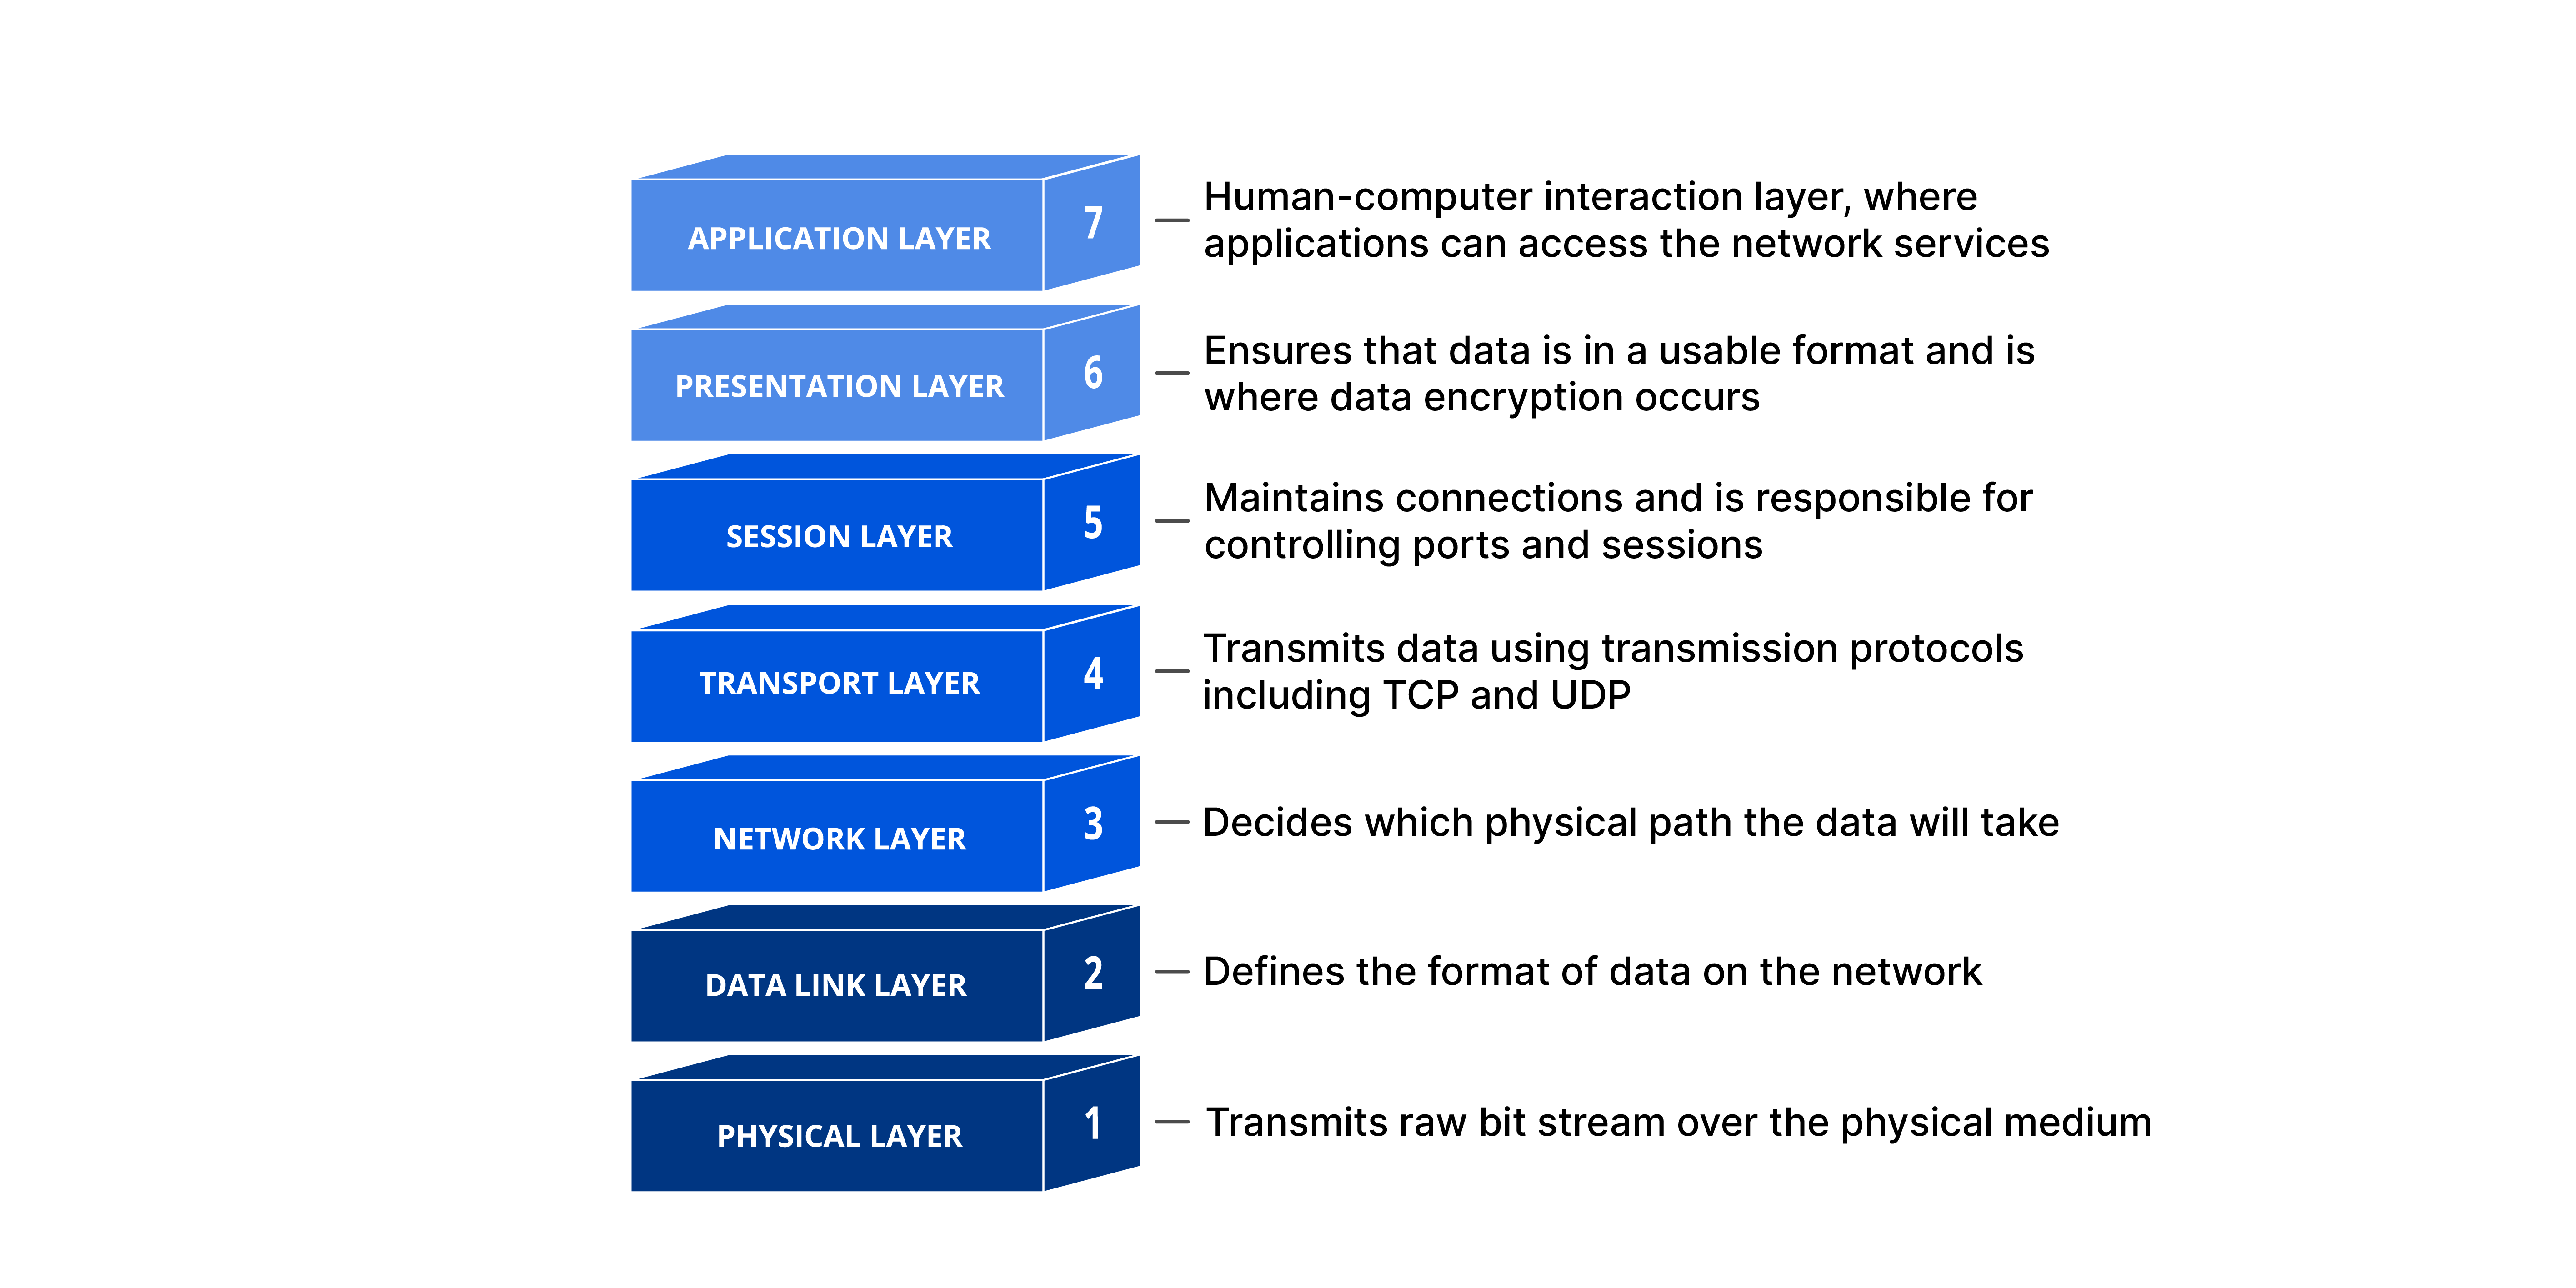
\includegraphics[width=0.8\textwidth]{images/osi.png}
    \hfill
    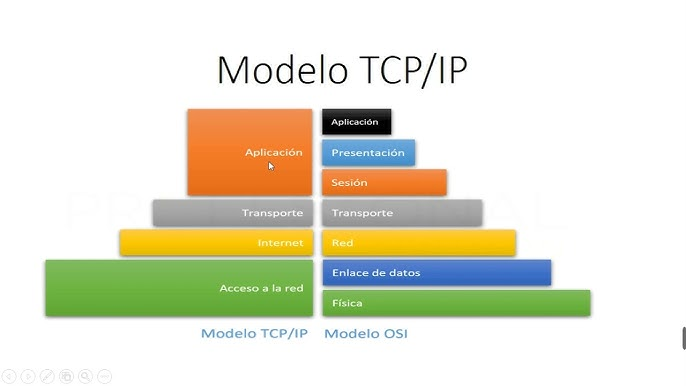
\includegraphics[width=0.8\textwidth]{images/TCP.jpg}
    \caption{Comparación entre el modelo OSI (izquierda) y el modelo TCP/IP (derecha).}
    \label{fig:models}
\end{figure}

\subsubsection*{¿Qué es un RFC?}

El término \textbf{RFC (Request for Comments)} se refiere a una serie de documentos que contienen especificaciones, estándares y directrices sobre cómo funciona Internet y sus protocolos asociados. Estos documentos son gestionados por el \textit{RFC Editor} bajo la supervisión del \textit{Internet Engineering Task Force (IETF)}.

\begin{itemize}
    \item Los RFC pueden describir protocolos como HTTP, TCP, IP, entre otros.
    \item También incluyen métodos, tecnologías y recomendaciones para la evolución de la arquitectura de Internet.
\end{itemize}

Por ejemplo, el \textbf{RFC 2026} detalla el procedimiento de normalización para los estándares de Internet. Los RFC son esenciales para asegurar que dispositivos y sistemas de diferentes fabricantes puedan comunicarse de forma eficiente y uniforme.

\subsection{Terminología, conceptos y servicios}

\begin{figure}[H]
    \centering
    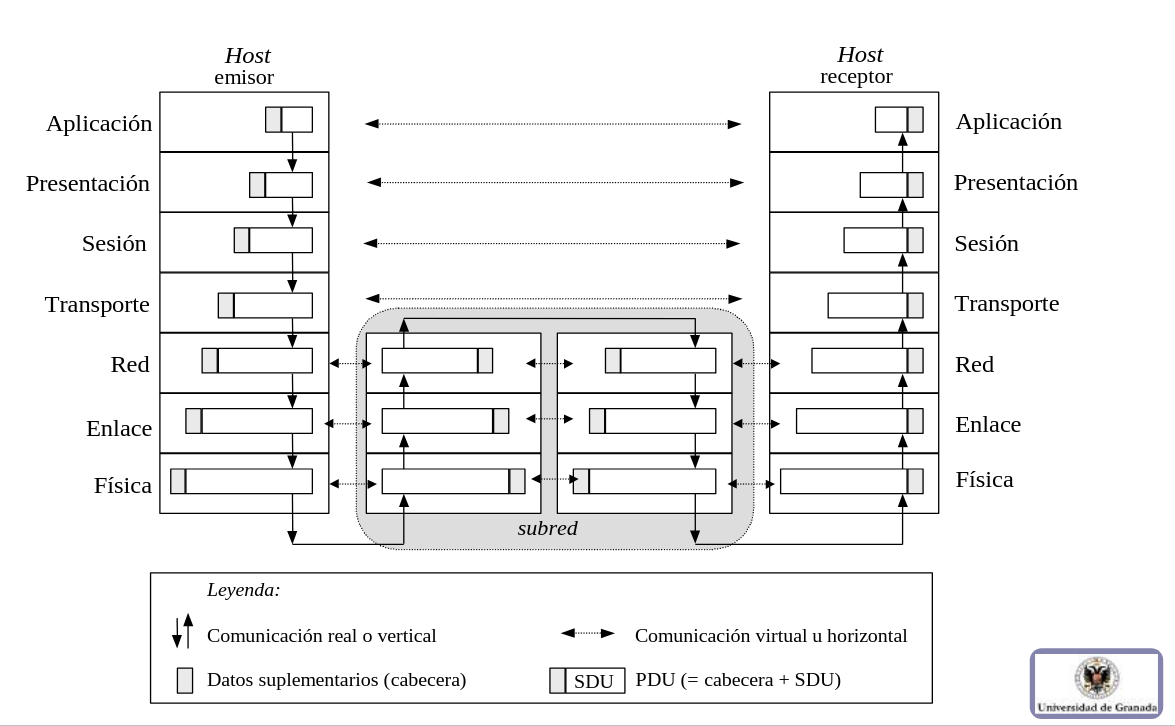
\includegraphics[width=1\textwidth]{images/osi_comparacion.png}
    \caption{Terminología y conceptos básicos en redes de computadoras.}
    \label{fig:terminology}
\end{figure}

\subsubsection*{Terminología, Conceptos y Servicios}

La terminología y los conceptos relacionados con las redes son esenciales para comprender cómo los dispositivos interactúan y cómo se estructuran las comunicaciones. A continuación, se detallan los términos principales:

\paragraph{Comunicación real (vertical):}
Es el intercambio de datos que ocurre entre capas adyacentes dentro de un dispositivo. Esta comunicación sigue un flujo descendente (del emisor) y ascendente (del receptor), en función del modelo de referencia utilizado.

\paragraph{Comunicación virtual (horizontal):}
Es la interacción lógica entre entidades pares en capas equivalentes de los dispositivos emisores y receptores. Aunque esta comunicación es conceptual, es facilitada por las capas inferiores.

\paragraph{Entidad del nivel N:}
Se refiere a una unidad funcional en la capa \(N\) del modelo OSI o similar. Por ejemplo, una entidad de la capa de transporte podría ser el protocolo TCP.

\paragraph{Entidades pares:}
Son entidades ubicadas en la misma capa de distintos dispositivos que se comunican mediante protocolos.

\paragraph{Protocolo:}
Es un conjunto de reglas que define cómo las entidades pares deben comunicarse. Incluye formatos, tiempos y secuencias de mensajes.

\paragraph{Interfaz:}
Es el punto de contacto entre capas adyacentes dentro de un dispositivo. Define cómo una capa accede a los servicios ofrecidos por la capa inferior.

\paragraph{Servicio:}
Es la funcionalidad que una capa provee a la capa superior. Por ejemplo, la capa de transporte ofrece servicios de entrega confiable a la capa de aplicación.

\paragraph{Capa proveedora y capa usuaria:}
La capa proveedora es aquella que ofrece un servicio, mientras que la capa usuaria lo consume. Por ejemplo, la capa de red es proveedora de la capa de transporte.

\paragraph{Pila de protocolos:}
Es la implementación de los protocolos en cada capa, que trabaja conjuntamente para permitir la comunicación de extremo a extremo.

\paragraph{Arquitectura de red:}
Es la combinación de un modelo de referencia (como OSI) y una pila de protocolos que define cómo funciona la red.

\paragraph{SAP (Service Access Point):}
Es un punto en la interfaz entre capas donde una capa accede a los servicios de otra. Se usa para identificar el punto de interacción.

\paragraph{SDU (Service Data Unit):}
Es la unidad de datos que una capa recibe de la capa superior para procesar y transmitir.

\paragraph{PDU (Protocol Data Unit):}
Es la unidad de datos intercambiada entre entidades pares en una capa. Incluye la SDU y cualquier información de encabezado o pie agregada por la capa.

\begin{figure}[H]
    \centering
    % Sustituye 'ruta_a_la_imagen.png' con la ruta de tu imagen
    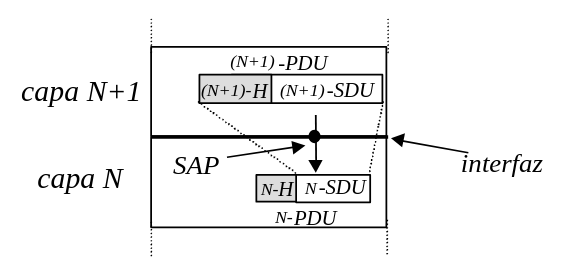
\includegraphics[width=0.5\textwidth]{images/capanycapanmas1.png}
\end{figure}

Estos conceptos son fundamentales para garantizar el \textit{intercambio de información transparente} entre los hosts, proporcionando una base sólida para entender cómo operan las redes modernas.

\subsubsection{Retardos en la comunicación}

\subsubsection*{Fórmulas}

Tiempo de transmisión:

\begin{equation}
    T_t = \frac{L}{V_t}
\end{equation}

Tiempo de propagación:

\begin{equation}
    T_p = \frac{D(m)}{V_t(m/s)}
\end{equation}

\begin{figure}[H]
    \centering
    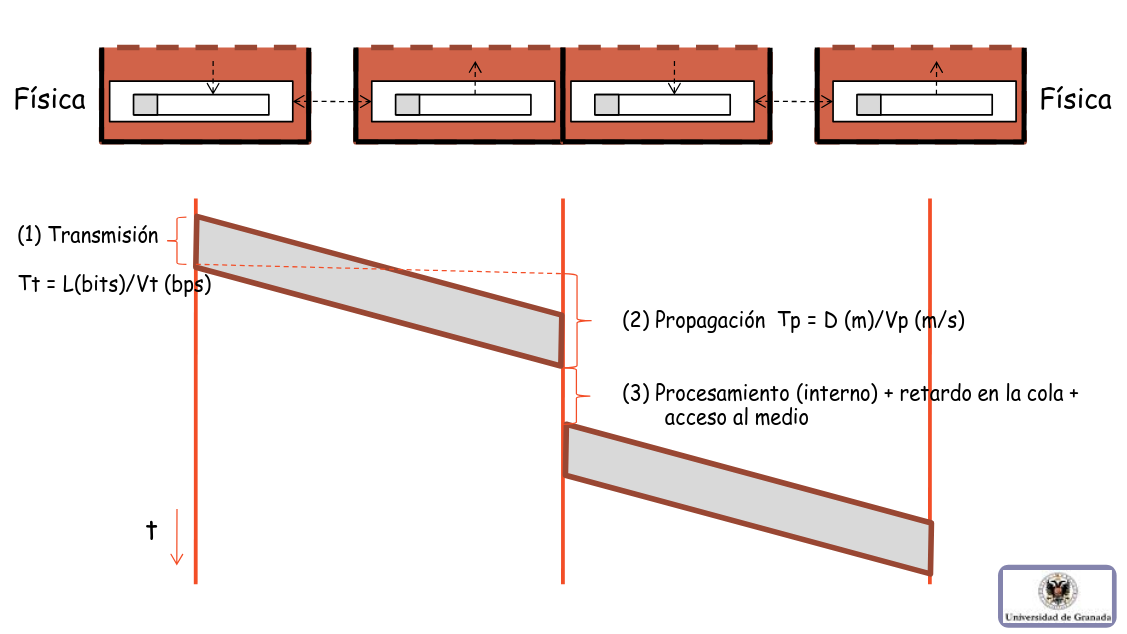
\includegraphics[width=0.8\textwidth]{images/RetardosComunicacions.png}
\end{figure}

%tcolorbox

\begin{tcolorbox}[colback=green!5!white, colframe=green!75!black, title=Nota]
    Si usamos la orden \textbf{ping} de una dirección, como por ejemplo de \textit{www.google.com}, podemos obtener el tiempo de ida y vuelta de los paquetes.
\end{tcolorbox}

%diapositiva 27, que en mi tablet es la 22
% https://chatgpt.com/c/67693401-0fdc-8012-8dea-a3b6f3ca0d4a
\end{document}
